
\begin{figure*}[t]
\begin{subfigure}[b]{0.30\textwidth}
\centering
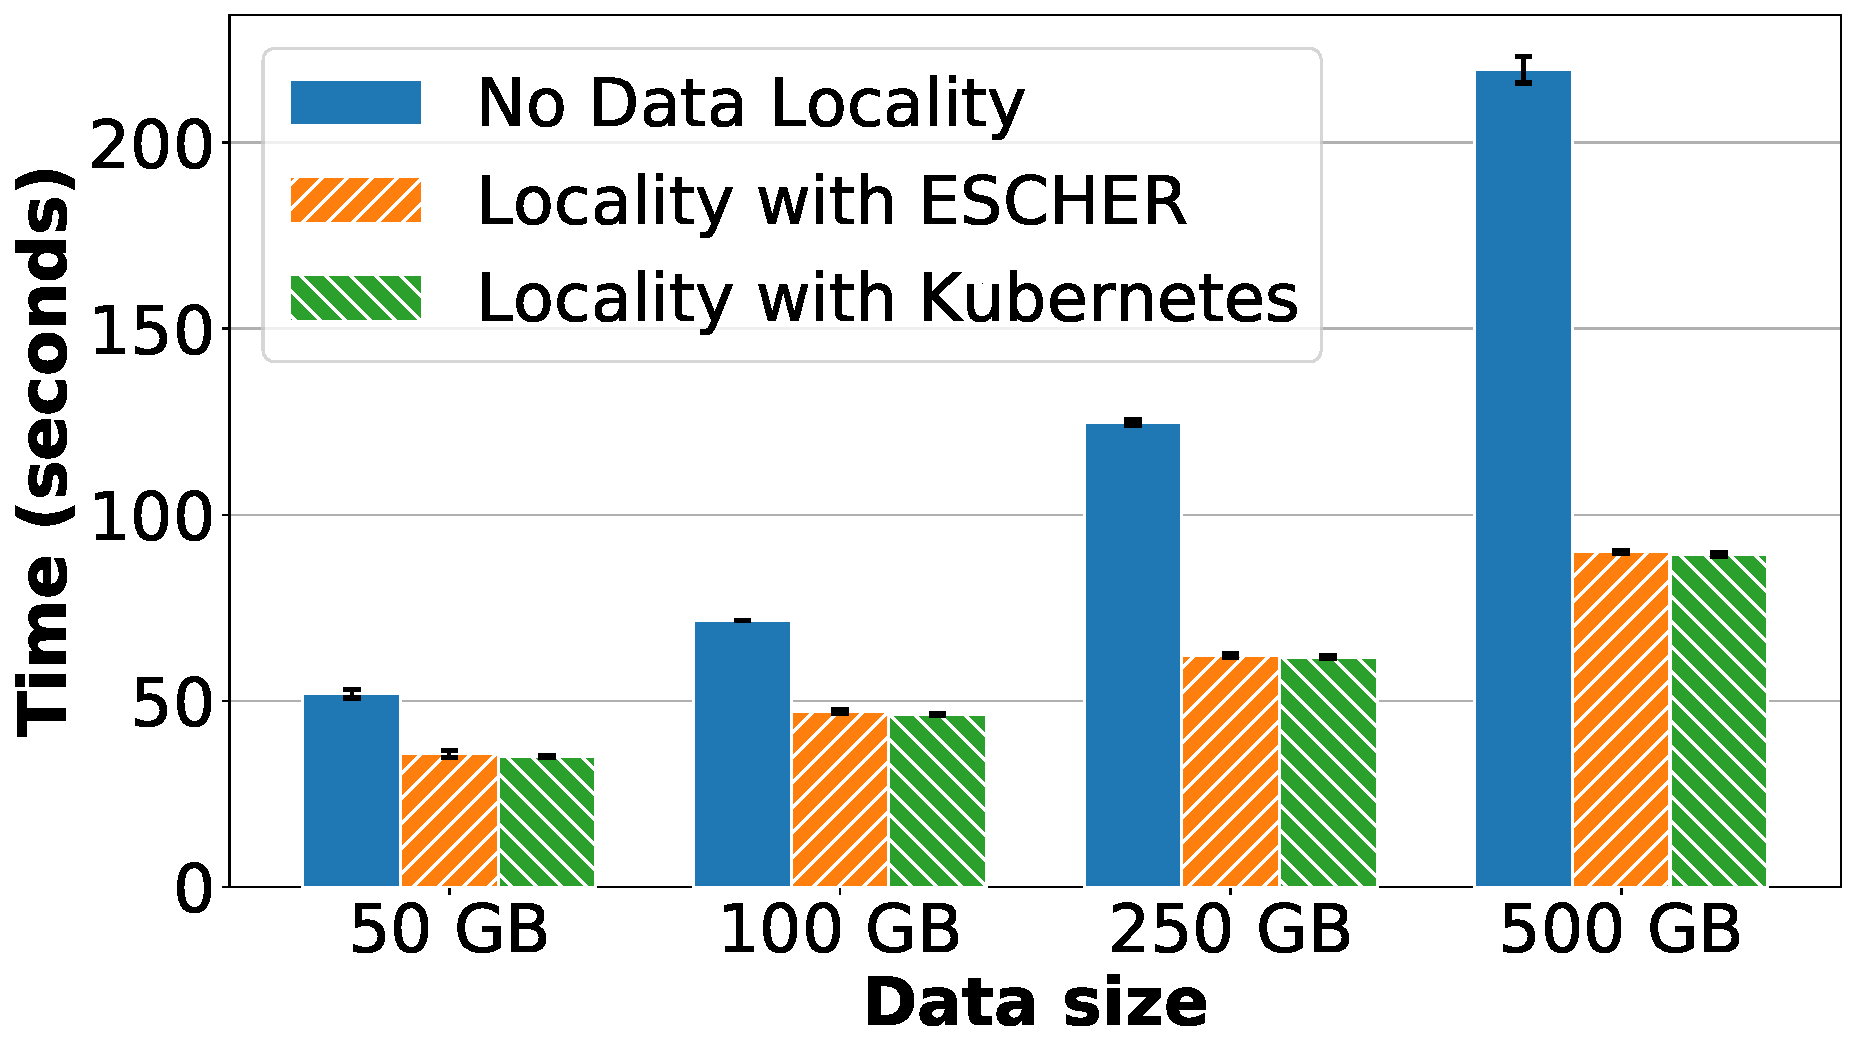
\includegraphics[width=\textwidth]{escher/plots/mapreduce_makespan.pdf}
\caption{
%A random placement policy has high network overheads due to poor data-locality. ESCHER implementation on Kubernetes performs comparably with the off-the-shelf core Kubernetes data locality policy.
}
\label{fig:mapreduce-makespan}
\end{subfigure}
\begin{subfigure}[b]{0.39\textwidth}
\hspace{2mm}
\footnotesize
% \begin{table}[ht]
% \begin{center}
\raisebox{15mm}{
\begin{tabular}{cccc}
% {\tiny
\toprule
& \multicolumn{3}{c}{\textbf{Scheduler}}\\
\textbf{Nodes}     & Generic & Kubernetes & ESCHER \\
\midrule
10 & $183.32 \pm 0.51$ & $54.69 \pm 0.46$ & $55.24 \pm 0.39$ \\\hline
50 & $113.71 \pm 0.49$ & $44.02 \pm 0.27$ & $44.71 \pm 0.44$  \\\hline
100 & $51.90 \pm 0.31$ & $35.08 \pm 0.31$ & $35.76 \pm 0.49$  \\
\bottomrule
% }
\end{tabular}
}
\caption{
% As the cluster size increases, ESCHER scales similarly to core kubernetes scheduler, while outperforming the generic data-locality unaware scheduler.
}
\label{tab:mapreduce-xnode}
%\vspace{-8mm}
% \end{table}
\end{subfigure}
\begin{subfigure}[b]{0.30\textwidth}
 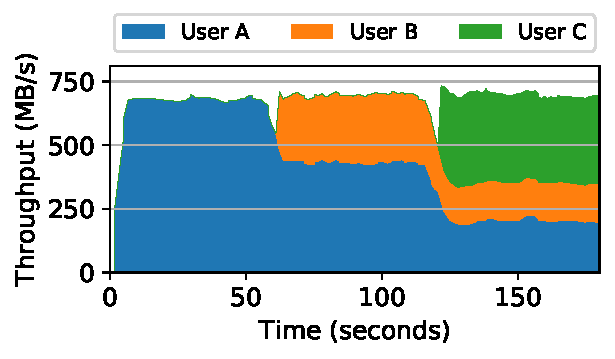
\includegraphics[width=\textwidth]{escher/plots/hfs/3user_hfs_sharing_mapreduce_50nodes_area_short.pdf}
 \caption{}
 \label{fig:hfs-3user-result}
\end{subfigure}
\vspace{-2em}
\caption{\small 
Data locality and hierarchical max-min fair sharing for WordCount.
\textbf{(a)} Makespan of WordCount running on a 100-node Kubernetes cluster, comparing a random placement policy, ESCHER on Kubernetes with data locality, and Kubernetes' native data locality.
\textbf{(b)} Makespan of WordCount MapReduce jobs in seconds across varying cluster sizes.
\textbf{(c)} Hierarchical max-min fair sharing with ESCHER.
A and B are in Sub-Org1 with weights 2:3; C is in Sub-Org2.
A, B, and C begin submitting tasks at $t=$0, 60, and 120, respectively.
}
\vspace{-3mm}
\end{figure*}


\section{Evaluation}
\label{sec:eval}

In this section, we evaluate the following questions:
\begin{compactitem}
    \item Can existing distributed applications be ported to use ESCHER and what are its implications?
    \item What are the tradeoffs with implementing scheduling policies in the application space vs in the framework?
    \item What are the overheads of scheduling with ephemeral resources?
\end{compactitem}

All evaluations use Amazon EC2 m5.12xlarge, m5.4xlarge or p3.8xlarge instances. Kubernetes clusters are provisioned using Amazon EKS running version 1.19.

\subsection{End-to-end Evaluation}
\label{sec:eval:e2e}
% Logical resources act as a thin layer of scheduling indirection for applications without sacrificing framework flexibility.
%In this section, we study four applications and their scheduling requirements. We then demonstrate how \name{} can accelerate these applications by allowing them to express complex scheduling policies with minimal developer effort.

\subsubsection{WordCount with MapReduce}
\label{eval:wordcount}
% What is mapreduce, what is word count
%These chunks are then individually processed by multiple mapper tasks in a distributed fashion. The results of mapper tasks are consumed by reduce tasks which key-wise consolidate the results.
WordCount counts the number of words in large text datasets and is often implemented with MapReduce~\cite{mapreduce}. To avoid expensive data transfers, data locality is essential.
% A data locality policy is essential to performance in this model, since map tasks must be colocated with their assigned inputs (which are usually on disk at a particular node) to avoid expensive data transfers.
% WordCount is a program implemented on the MapReduce~\cite{mapreduce} model to count the number of words in large text datasets. WordCount works by splitting the text file into smaller chunks, distributing them over the network and then running distributed mappers to count word frequency in these chunks.
% How data locality plays in. Implementation, HDFS Spark etc.
% The map tasks in WordCount are highly dependent on their locality with the data chunk they are assigned to process. If the data chunk is not present on the node where the map task is scheduled, it is forced to perform an expensive fetch over the network before starting processing. This dependence makes WordCount a benchmark to stress data-locality.
% Describe setup 100 nodes.
We implement the map and reduce tasks as independent operators running in containers.
The input files are chunks of a file with random words, each hosted by one of 100 nodes. The total input size is varied from 50 GB to 500 GB.
% and use Kubernetes to distribute these tasks over a 100-node cluster.
% The inputs are chunks of a file with random words, each  hosted by one of 100 nodes. 
% The total input size is varied from 50 GB to 500 GB.
%In this setup, the scheduler must place the mapper tasks on the nodes which host their chunk to minimize delays from network transfers.
We implement \name{} on Kubernetes, using an ESL for data locality (\Cref{policies}), and compare against Kubernetes's built-in data-locality policy~\cite{kubernetes-doc} and a locality-unaware random policy.
% For \name{} on Kubernetes, we use an ESL that implements data locality (\Cref{policies}).

% How do it in k8s, ESCHER.
% To achieve this data locality with the default Kubernetes scheduler, we use the \lstinline{NodeAffinityPriority} specifier in the scheduler to place mappers on nodes where their assigned chunk exists. This serves as a baseline to compares against ESCHER. In ESCHER, we create a resource \lstinline{chunk-n} on each node, where $n$ is the id of chunk hosted by the node. The mappers then request this resource to get co-located with their chunk. This policy is wrapped in an ESL which is invoked by WordCount.

Unsurprisingly, \Cref{fig:mapreduce-makespan} shows that as the input size increases, 
%the overhead of data transfer dominates execution if locality is not considered.
the overhead of transferring chunks over the network dominates the mapper computation time for the no-locality policy, taking up to 58.3\% of the total job time when the input size is 500 GB.
Meanwhile, \name{} on Kubernetes provides the same performance as Kubernetes itself, but without modifying the core scheduler framework.
Furthermore, \Cref{tab:mapreduce-xnode} shows that \name{} can also scale with the cluster size. 
%As the cluster size increases, the scheduling sub-system is stressed to distribute more map and reduce tasks.
Throughout different scales, ESCHER performs comparably with the core Kubernetes scheduler, with its makespan staying within $1.9\%$ of the baseline Kubernetes scheduler.. Implementing data locality with ESCHER required adding only two lines:  a \lstinline{set_resource} call during data generation to create a local \lstinline{data-<id>} resource and a line to specify a \lstinline{data-<id>} resource requirement for the mapper tasks.

% Compares against k8s
% Figure \ref{fig:mapreduce-makespan} and \Cref{tab:mapreduce-xnode} compare the makespan across different input and cluster sizes. % for a scheduling policy implemented in ESCHER, the off-the-shelf data-locality scheduler in Kubernetes and a policy which randomly places mappers without any data-locality.
% As the input size increases, the overhead of transferring chunks over the network dominates the mapper computation time for the no-locality policy, taking up to 58.3\% of the total job time when the input size is 500 GB.
% \Cref{fig:mapreduce-makespan} shows that ESCHER on Kubernetes can provide the same application-level benefits as Kubernetes itself, but without modifying the core scheduler framework.
% Furthermore, \Cref{tab:mapreduce-xnode} shows that as the cluster size increases, ESCHER can also scale with the increased number of map and reduce tasks (within $1.9\%$ of the core Kubernetes scheduler).

% As the cluster size increases, the scheduling sub-system is stressed to distribute more map and reduce tasks. Throughout different settings, ESCHER performs comparably with the core Kubernetes scheduler, with its makespan staying within $1.9\%$ of the baseline Kubernetes scheduler. 



% \begin{figure}
% \centering
% 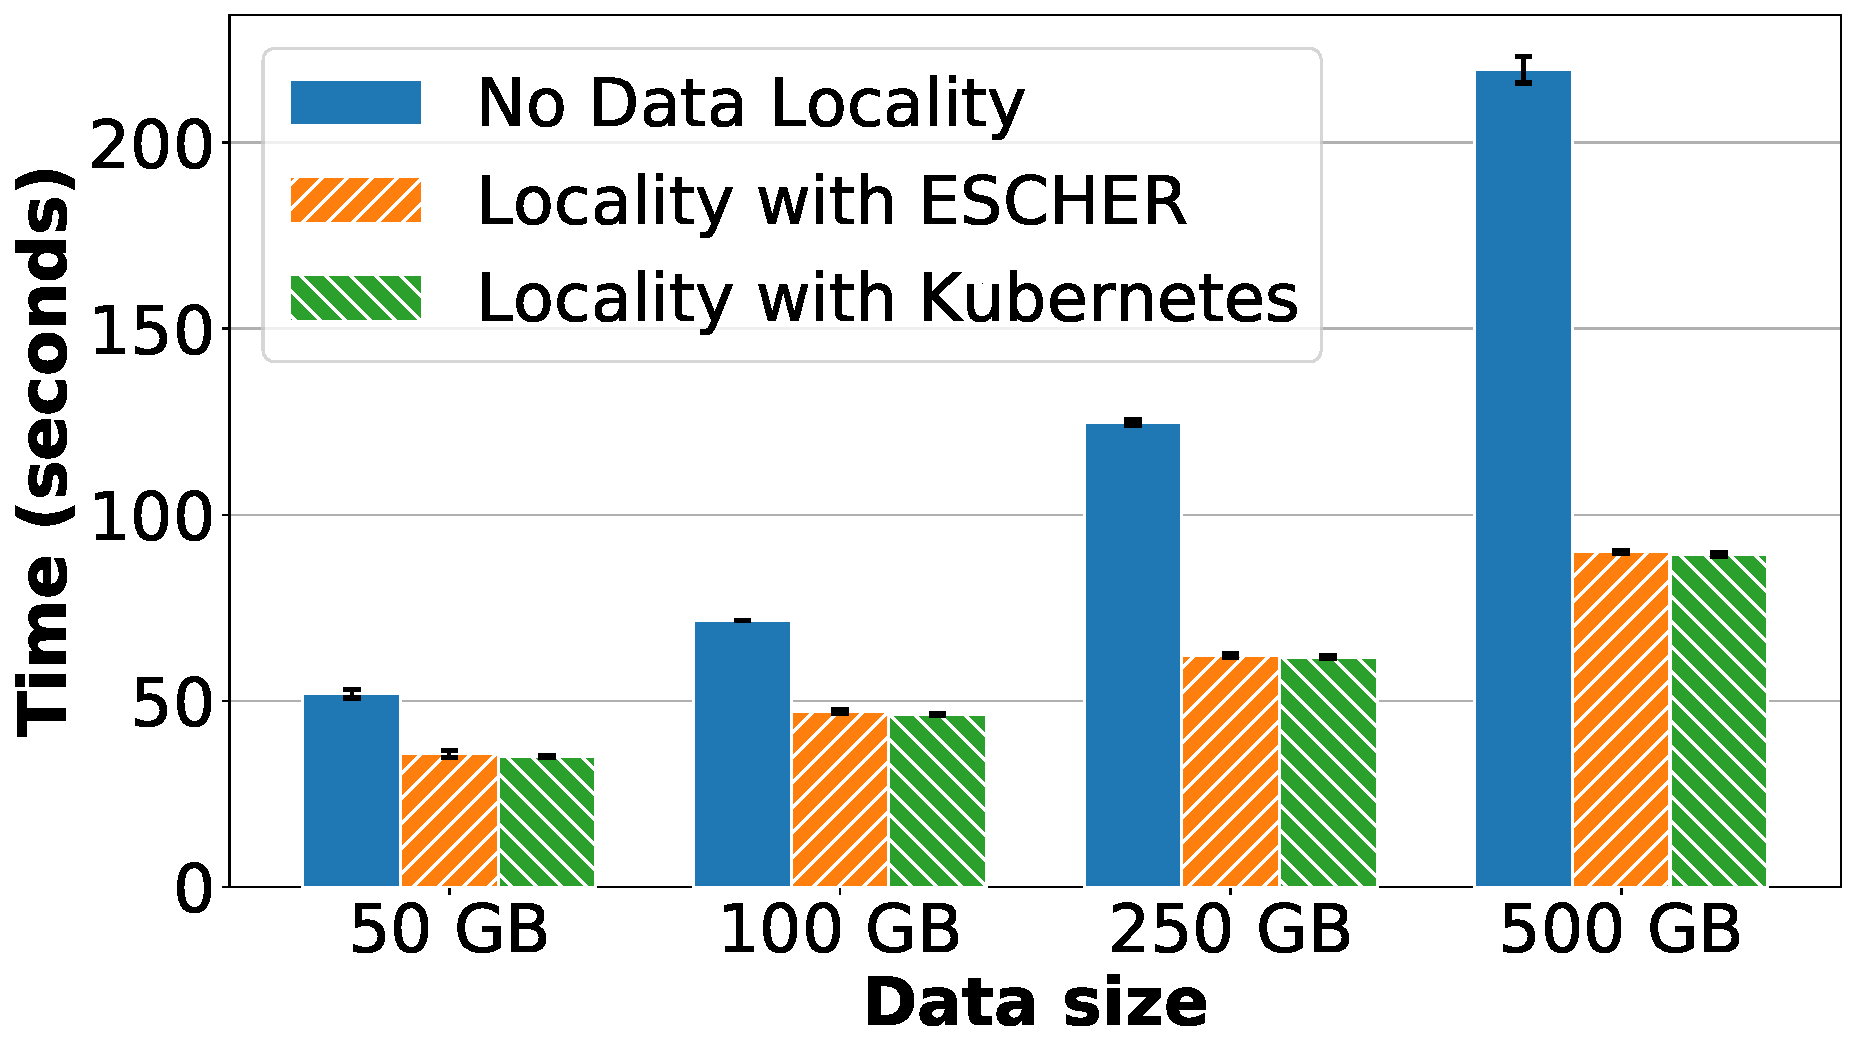
\includegraphics[width=0.8\columnwidth]{escher/plots/mapreduce_makespan.pdf}
% \caption{\small Makespan of WordCount running on a 100-node Kubernetes cluster, comparing a random placement policy, ESCHER on Kubernetes with data locality, and Kubernetes' native data locality.
% %A random placement policy has high network overheads due to poor data-locality. ESCHER implementation on Kubernetes performs comparably with the off-the-shelf core Kubernetes data locality policy.
% }
% \label{fig:mapreduce-makespan}
% \end{figure}

% \begin{table}[ht]
% \begin{center}
% \begin{tabular}{cccc}
% \toprule
% & \multicolumn{3}{c}{\textbf{Scheduler}}\\
% \textbf{Nodes}     & Generic & Kubernetes & ESCHER \\
% \midrule
% 10 & $183.32 \pm 0.51$ & $54.69 \pm 0.46$ & $55.24 \pm 0.39$ \\\hline
% 50 & $113.71 \pm 0.49$ & $44.02 \pm 0.27$ & $44.71 \pm 0.44$  \\\hline
% 100 & $51.90 \pm 0.31$ & $35.08 \pm 0.31$ & $35.76 \pm 0.49$  \\
% \bottomrule
% \end{tabular}
% \end{center}
% \caption{\small Makespan of WordCount MapReduce jobs in seconds, compared across varying cluster sizes.
% % As the cluster size increases, ESCHER scales similarly to core kubernetes scheduler, while outperforming the generic data-locality unaware scheduler.
% }
% \label{tab:mapreduce-xnode}
% %\vspace{-8mm}
% \end{table}


% \begin{figure}[ht]
% % \begin{subfigure}{1\linewidth}
% % \centering
% % 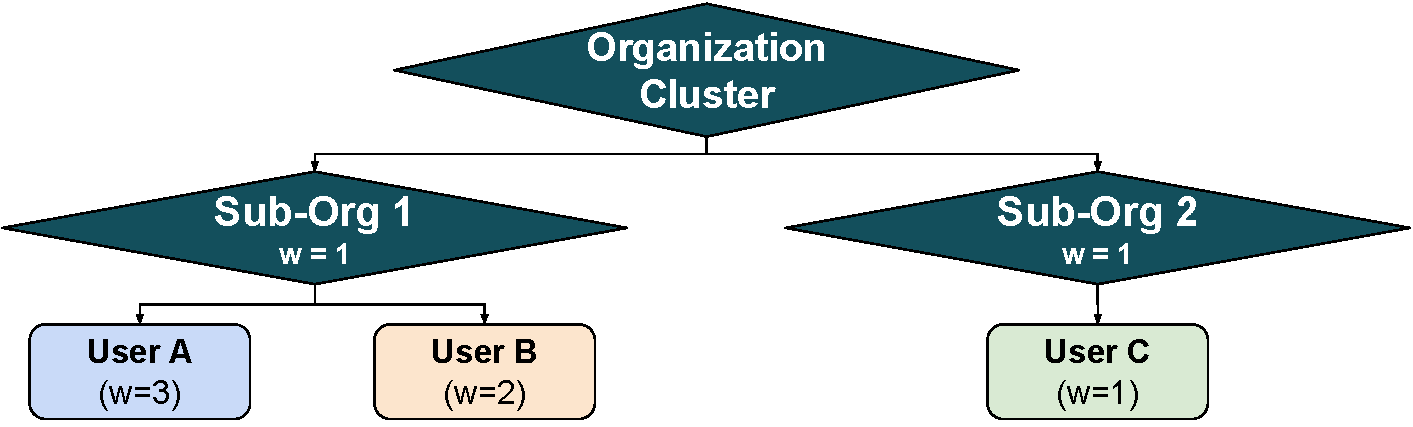
\includegraphics[width=1\columnwidth]{escher/plots/hfs/ESCHER_HFS_3User_OrgChart.pdf}
% % \caption{Organization Chart}
% % \label{fig:hfs-3user-orgchart}
% % \end{subfigure}
% % \begin{subfigure}{1\linewidth}
% \centering
% 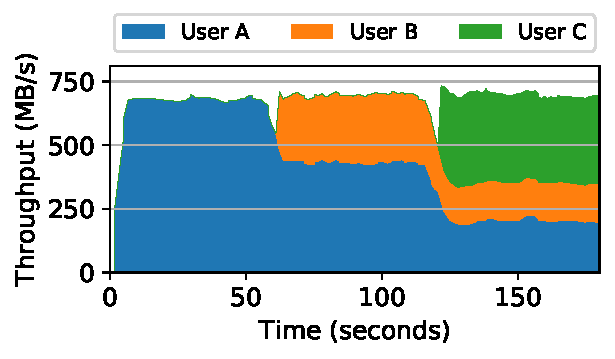
\includegraphics[width=0.93\columnwidth]{escher/plots/hfs/3user_hfs_sharing_mapreduce_50nodes_area_short.pdf}
% % \caption{User-wise throughput}
% % \end{subfigure}
% \caption{\small Per-user WordCount throughput with hierarchical max-min fair sharing.
% A and B are in Sub-Org1 with weights 2:3; C is in Sub-Org2.
% A, B, and C begin submitting tasks at $t=0,60,120$, respectively.
% %(a) shows the organization chart for resource sharing between sub-org 1 and sub-org 2. Weights (w) are relative to other users under the same parent.
% % (b) plots the throughput for users A, B and C on a cluster of 50 nodes.
% %At time t=0, only user A is submitting tasks so the HFS ESL allocates all resources to user A. At time t=60 and t=120, User B and User C start submitting tasks respectively.
% % The HFS ESLs adjust resource allocations based on utilization while maintaining organization level and sub-organization level weight proportional fairness.
% }
% \label{fig:hfs-3user-result}
% \end{figure}
% Two interfaces - infeasible and cancel tasks
% Throughput bug

% \begin{figure}
% \begin{subfigure}{1\linewidth}
% \centering
% 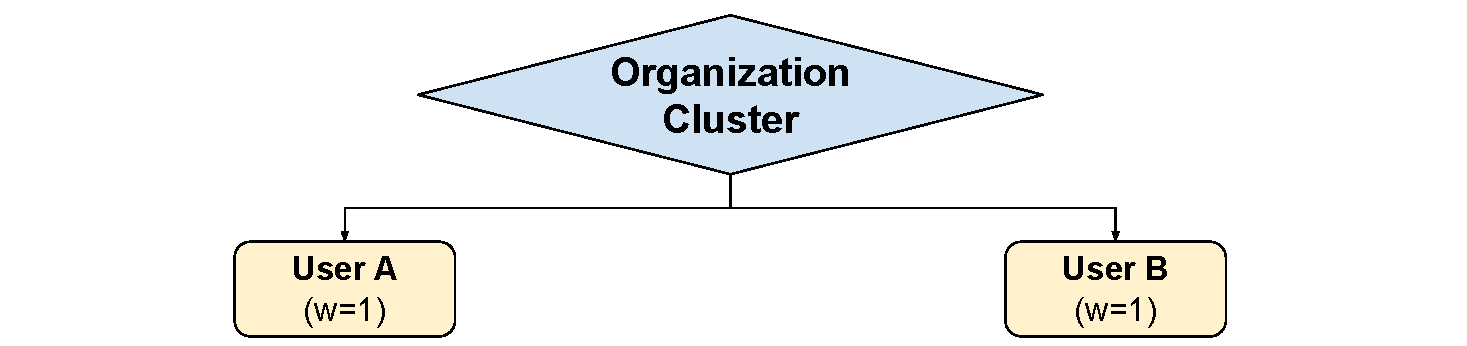
\includegraphics[width=1\columnwidth]{escher/plots/hfs/ESCHER_HFS_2User_OrgChart.pdf}
% \caption{Organization Chart}
% \label{fig:hfs-2user-orgchart}
% \end{subfigure}
% \begin{subfigure}{1\linewidth}
% \centering
% 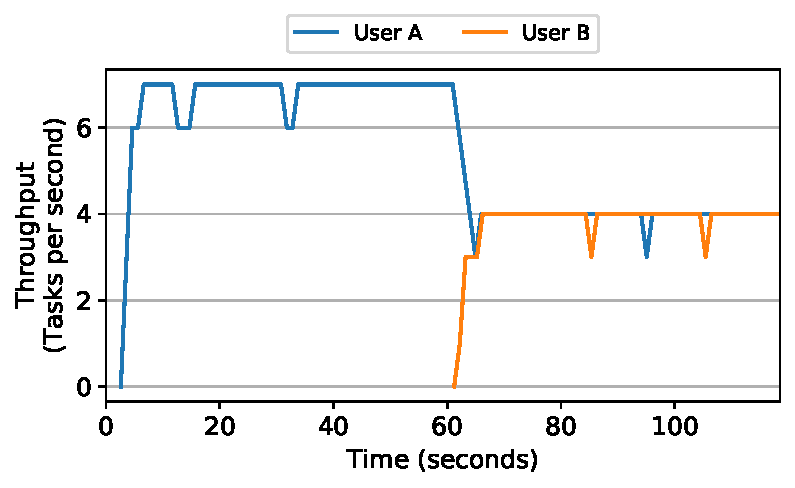
\includegraphics[width=0.9\columnwidth]{escher/plots/hfs/2user_hfs_sharing.pdf}
% \caption{User-wise throughput}
% \label{fig:hfs-2user-result}
% \end{subfigure}
% \caption{\small Min-Max Fair Sharing with ESCHER. Figure (a) shows the organization chart for resource sharing between User A and User B, each having equal weights (w=1). Figure (b) plots the throughput for users A and B. At time t=0, only user A is submitting tasks so the HFS ESL allocates all resources to user A. At time t=60 user B starts submitting tasks. The HFS ESL adjusts deallocates resources from user A and reassigns them to user B to maintain fairness.  
% }
% \label{fig:hfs-2user}
% \end{figure}

\subsubsection{Hierarchical max-min fair sharing}
\label{eval:hfs}
% Cool bits:
% \begin{itemize}
%     \item The resizing of the cluster is completely transparent to the users - they don't need to worry how many resources are allocated to them
%     \item Composition of data locality and fair sharing is as simple as adding resource requirements.
% \end{itemize}
Hierarchical Max-Min Fair Sharing (\Cref{policies}) allocates resources proportionate to a user's weight in a hierarchical organization.
% HFS maximizes resource utilization by reallocating idle resources.
Users submit jobs at different times, so their ideal absolute resource share is dynamic, making it impossible to maximize overall resource utilization with static labels.
% This makes it impossible to implement HFS with a static label-based scheduler since the resource share per user is dynamic.
For example, consider a two-team organization: Sub-Org1 with users A and B of weights 2:3, and Sub-Org2 with user C.
% with equal weights - Sub-Org1 and Sub-Org2. Sub-Org1 has two users, A and B with weights 2:3, while sub-org2 has one user C.
To ensure fairness with static labels, the only option is to allocate each user a fixed proportionate share, leading to under-utilization when only one user is submitting work.

% To achieve fairness, the only option with static labels would be to allocate each user a fixed share, leading to under-utilization in \Cref{fig:hfs-3user-result}. (i.e., A would only reach 200MB/s at $t$=0).

Because ephemeral resources can be \emph{dynamically} created and destroyed, an HFS policy ensures fairness while also maximizing overall utilization as users enter and leave the system~(\Cref{fig:hfs-3user-result}).
We deploy a HFS policy on a 100 node cluster running WordCount. We use a parent ESL for the teams and two children ESLs for Sub-Orgs 1 and 2 to create a hierarchy of ESLs.
An HFS ESL tracks idle resources and reallocates resources between teams or users.
% For example, at $t$=60 in \Cref{fig:hfs-3user-result}, B begins submitting tasks, causing the Sub-Org1 ESL to reclaim resources from A.
The workload in \Cref{fig:hfs-3user-result} starts with only user A submitting tasks to the scheduler. Since other users' resources are idle, the HFS ESLs re-allocate all idle resources to A to achieve max-min fairness. At time $t$=60, user B starts submitting tasks. This causes the Sub-Org 1 ESL to reclaim resources from A to re-allocate to B, in proportion to their weights. B's warmup time causes a small dip in net throughput at $t$=60. Finally at time $t$=120, user C starts submitting tasks and the parent ESL reallocates resources to Sub-Org2. Since Sub-Org 2 and Sub-Org 1 have equal weights, C's resource allocation is equal to the sum of A and B's allocation.
Ephemeral resources also enable composition: the application composes its custom policy (in this case, data locality for WordCount) with the two HFS ESLs by concatenating all the resource requirements.

% The workload in \Cref{fig:hfs-3user-result} starts with only user A submitting tasks to the scheduler. Since other users' resources are idle, the HFS ESLs re-allocate all idle resources to A to achieve max-min fairness. At time $t$=60, user B starts submitting tasks.
% This causes the Sub-Org 1 ESL to reclaim resources from A to re-allocate to B, in proportion to their weights. B's warmup time causes a small dip in net throughput at $t$=60. Finally at time $t$=120, user C starts submitting tasks and the parent ESL reallocates resources to Sub-Org2. Since Sub-Org 2 and Sub-Org 1 have equal weights, C's resource allocation is equal to the sum of A and B's allocation.

% Not only is ESCHER able to maintain the cluster's fair-sharing requirements, it also allows the each user to compose their application-level policies with cluster-level policies. This is achieved by simply concatenating the data-locality resources with the resource requirement vector from the fair-sharing ESL. This concatenation ensures that the scheduler places the tasks where both constraints - fairness and data-locality - can be satisfied.

% Using ephemeral resources also reduces implementation complexity by enabling transparent resizing of user shares when applying max-min fairness. Since the ESLs dynamically create and removes each user's ephemeral resources from underlying nodes, the users' applications are not required to keep a track of the resources allocated to them. This would not have been possible in a static label-based scheduler since the max-min shares for each user are dynamic. 



\subsubsection{AlphaZero}
AlphaZero \cite{silver2017mastering} is a reinforcement learning application for the board game Go.
%Unlike it's predecessor AlphaGo\cite{silver2016alphago}, AlphaZero does not require any human-generated training samples and can instead leverage reinforcement learning techniques to play and learn from games against itself.
%We base this experiment off an existing AlphaZero implementation \cite{anthony2017thinking}, which uses hard-coded process placement.
We demonstrate \name{}'s flexibility by porting an implementation~\cite{anthony2017thinking} onto Ray without compromising performance relative to the optimal hard-coded (but inflexible) placement.

AlphaZero executes a Monte Carlo Tree Search on the game state space in a CPU-intensive \textit{BoardAggregator} process. The search is guided by a \textit{PredictorAgent} running a neural network on a GPU which evaluates a board and predicts the associated reward.
%Based on this prediction, the \textit{BoardAggregator} generates new boards to explore and learn from.
% This pattern creates a tight feedback loop between the \textit{BoardAggregator} and the \textit{PredictorAgent}.
Co-locating \textit{BoardAggregator}s and their corresponding \textit{PredictorAgent}s on the same physical node is thus desirable to avoid network overheads from transferring board states. These pairings also require anti-affinity for load balancing and to avoid interference \cite{gandiva}.
%Many existing frameworks do not allow the expression of this composition of load-balancing and co-location policies, while others frameworks would require a tedious re-implementation of the scheduler. 
With ephemeral resources, this composed policy can be specified in 5 lines of code~(\cref{fig:alphazerocode}): we apply a load-balancing policy~(\Cref{tab:escher-constraints-policies}) to the \textit{PredictorAgent} and a co-location policy to the \textit{BoardAggregator} and \textit{PredictorAgent}.
%This composition takes only 5 lines of code (\cref{fig:alphazerocode}).

We ran 10k iterations of AlphaZero on a 32-node cluster (128 GPUs total). %board generation distributed across 16 machines with a total of 128 GPUs.
We compare three setups: 
(a) co-location with hard-coded placement,
(b) co-location with ephemeral resources, and 
(c) a baseline policy with no co-location. 
\Cref{fig:alphazerolatencycdf} plots the CDF for board exploration time. %, which includes generating the board on the \textit{BoardAggregator} and evaluating it on the \textit{PredictorAgent}. 
% Comparing the percentile distributions from this CDF in \cref{fig:alphazerolatencypxx}
Co-location is important for performance, outperforming no-colocation by 15.4\% in median latency and 20\% in P95 latency. %, demonstrating the benefits of co-location.
Additionally, co-location with ephemeral resources adds insignificant overheads of <1\%, while requiring less developer effort: the application code~(\Cref{fig:alphazerocode}) does not need to match \textit{PredictorAgent}-\textit{BoardAggregator} pairs to specific nodes.

% while providing a much simpler interface to express scheduling requirements.

%and by 714\% on P99.9 latency. P99.9 latency demonstrates the largest difference because the initial queries in the no-colocation case require setting up inter-machine communication sockets which may take time.

% Co-location with Logical Resources Stats - P999: 0.05949, P95: 0.02135, P50: 0.02083
% Static Co-location Stats - P999: 0.05863, P95: 0.02147, P50: 0.02079
% No Co-location Stats - P999: 0.06227, P95: 0.02578, P50: 0.02401


% \begin{figure}
% ~
% % Task co-location
% ~
% \begin{subfigure}{.22\textwidth}
%   \centering
%   \begin{minted}[fontsize=\tiny,breaksymbolleft=\tiny\ensuremath{},breakautoindent=true]{python}
% class PredictorAgent():
%   def __init__(id):
%     # Create resource for co-location
%     set_resource(label=id, capacity=1)
%     ...
%   \end{minted}
% \end{subfigure}
% ~
% % Task co-location
% ~
% \begin{subfigure}{.22\textwidth}
%   \centering
%   \begin{minted}[fontsize=\tiny,breaksymbolleft=\tiny\ensuremath{},breakautoindent=true]{python}
% class BoardAggregator():
%   def __init__(predictor):
%     # Assign predictor handle
%     self.predictor = predictor
%     ...
%   \end{minted}
% \end{subfigure}

% \newline

% \begin{subfigure}{.49\textwidth}
%   \centering
%   \begin{minted}[fontsize=\tiny,breaksymbolleft=\tiny\ensuremath{},breakautoindent=true]{python}
% def main():
%     # Create load-balancing resources
%     for node in cluster:
%         set_resource("load_bal", 1, node)
%     for i in range(0, num_agents):
%         p = PredictorAgent(resources = {"GPU": 1, "load_bal": 1}).launch(id=i)
%         # The predictor creates a resource with label i
%         # This resource is used by the BoardAggregator to co-locate.
%         b = BoardAggregator(resources = {i: 1}).launch(predictor=p)
%   \end{minted}
% \end{subfigure}
% \caption{AlphaZero placement preferences with \name{}}
% \label{figure:alphago}
% \end{figure}

\subsubsection{Distributed Training}
\label{sec:eval:tune}


% \begin{figure}
% 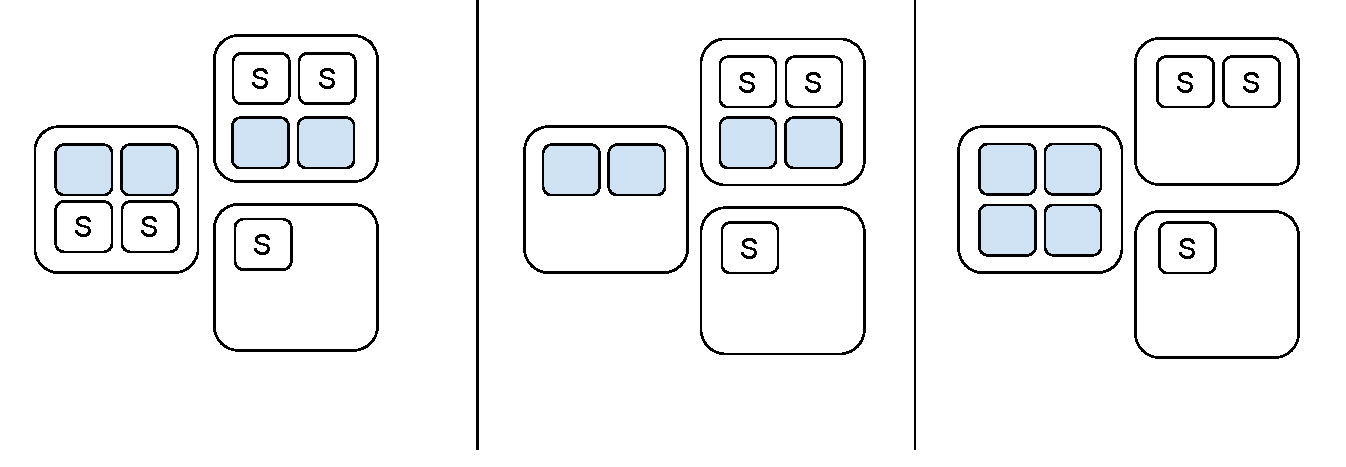
\includegraphics[width=0.9\columnwidth]{escher/figures/Eschertune.pdf}
% \caption{Migration after termination of the Short Job, signaling EscherTune to utilize a co-location mechanism and decrease communication overhead compared to Tune.
% }
% \label{fig:tune-results}
% \end{figure}



\def\longjob{\emph{long-job}}
\def\shortjobs{\emph{short-jobs}}
% Distributed training for a ML model typically consists of multiple workers that compute model updates in parallel and in lockstep.
For a distributed training job, worker placement is critical to performance, as co-locating workers reduces the cost of model synchronization at each step.
% The placement of these workers in a cluster is critical to the performance of the training process, as co-located workers avoid the network cost of model synchronization on each update operation.
%Typically, multiple jobs, each with different size and unpredictable completion time, will execute in parallel as part of a hyperparameter search~\cite{liaw2018tune}.
% Moreover, training jobs in a shared cluster can be of different sizes and with unpredictable completion times.
Gandiva \cite{gandiva} is a scheduler for deep learning jobs that aims to optimize training job performance. It composes a higher level \textit{load-balancing} policy and a lower-level \textit{co-location} policy to evenly spread jobs across machines while reducing intra-job communication overhead. 
To demonstrate \name{}'s flexibility, we augment Gandiva's \cite{gandiva} worker co-location and migration policy with Gang Scheduling to support distributed training jobs, and integrate the policy into Tune \cite{liaw2018tune}, an open source distributed training library built on Ray \cite{ray-osdi}, which we will refer to as \textit{EscherTune}.
We modified the Trial abstraction in Tune to be wrapped in a ghost task that ensures gang scheduling and applied co-location on tasks belonging to the same Trial.
%EscherTune records the current cluster placements during execution.
EscherTune triggers a migration whenever it detects sufficient available resources to place all workers of a job on the same node.
To execute a worker migration, EscherTune checkpoints the current job using application-specific checkpoint functionality and destroys all current workers. Then, EscherTune assigns ephemeral resources to the new target node, and relaunches all worker tasks of the training job without modifying their ephemeral resource requests.
 %To execute a worker migration, EscherTune will checkpoint the current training job using framework-dependent checkpoint functionality and destroy all current workers. Then, EscherTune assigns ephemeral resources to the target node and relaunches all worker processes of the training job with the specified ephemeral resource requests.
 
We compare EscherTune with Tune's open-source policy on a cluster of 12 GPUs. We launch 5 short-running training jobs (\shortjobs{}), each requiring 1 GPU, followed by 1 long-running training job requiring 4 GPUs (\longjob{}).
Each training job is training a ResNet-101 model on CIFAR-10 with a batch-size of 64 images per device.

Initially, the \shortjobs{} are load-balanced across the cluster, while the 4 workers of the \longjob{} are spread across the cluster depending on GPU availability. This is a sub-optimal placement, so EscherTune migrates the \longjob{} to colocate its tasks as soon as resources become available from a \emph{short-job} completion, resulting in 36.3\% higher throughput~(\Cref{fig:tune-results}).
Meanwhile, Tune uses a static placement, so the \longjob{}'s throughput remains the same.
% Figure \ref{fig:tune-results} compares throughput of \longjob{} in EscherTune and Tune, with all jobs launched at the same time. The throughput is low when the workers are spread across the cluster, but when there are sufficient resources to place workers on the same node, EscherTune is able to use ephemeral resources to migrate and co-locate all workers, increasing the throughput of the job by 36.3\%.
Furthermore, EscherTune's implementation consists of only 50 lines of Python, with no changes to Tune or the Ray scheduler. % a callback of 50 lines of Python, with \textit{no changes} to Tune.
 

% \begin{figure}[t]
% \centering
% 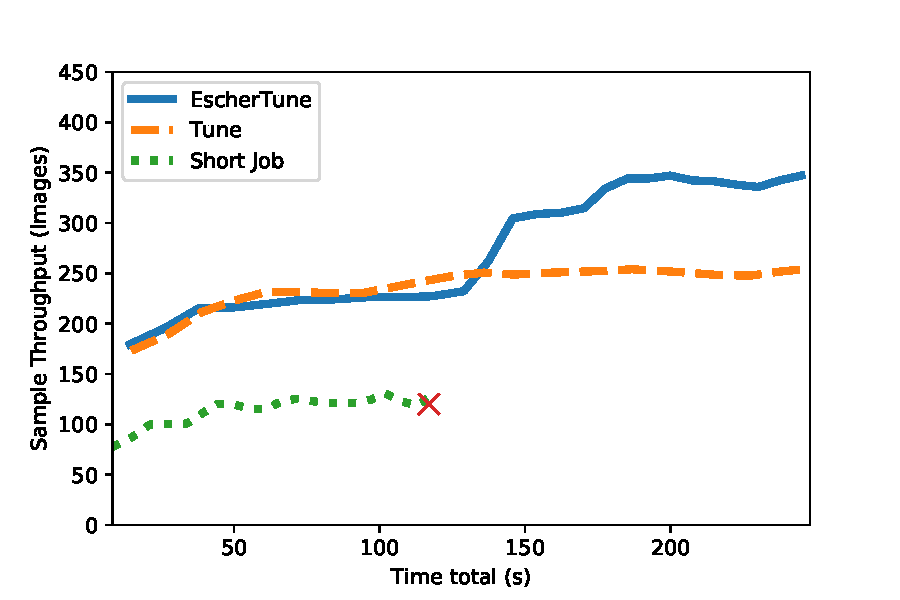
\includegraphics[width=0.85\columnwidth]{escher/plots/result_migrationthroughput.pdf}
% \caption{\small Throughput comparison of distributed training workloads with and without migration. ESCHER is able to augment an existing application, Tune, to increase sample throughput. 
% The red X indicates the termination of the short job, signaling EscherTune to utilize the co-location mechanism and decrease communication overhead compared to Tune.
% }
% % \caption{Throughput comparison of distributed training jobs with and without migration. 
% % Sample throughput for training can increase significantly by co-locating workers of
% % a distributed training job. In this mixed workload containing a distributed training job for a ResNet-101 architecture using 4 workers, ESCHER is able to easily augment the underlying framework to significantly improve performance. 
% % The red X indicates the termination of the Short Job, signaling EscherTune to utilize a co-location mechanism and decrease communication overhead compared to Tune.
% % }
% \label{fig:tune-results}
% \vspace{-0.3in}
% \end{figure}

% \subsubsection{Implementing Kube-Batch with ESCHER}
% To demonstrate ESCHER's ease-of-use, we add Gang Scheduling to Kubernetes using the Ephemeral Resources API and compare the implementation with a plug-in scheduler which adds this functionality to kubernetes. As described in Section \ref{sec:motivation}, adding gang scheduling to Kuberenetes in it's current form has been possible only through separate plug-in schedulers. One such plug-in is kube batch
\begin{figure*}[t]
\begin{subfigure}[b]{0.47\linewidth}
  \centering
\begin{subfigure}[t]{.22\textwidth}
  \centering
  \begin{minted}[fontsize=\tiny,breaksymbolleft=\tiny\ensuremath{},breakautoindent=true]{python}
class PredictorAgent():
  def __init__(id):
    # Create co-location resource.
    set_resource(
      name=id,
      capacity=1)
    ...
  \end{minted}
\end{subfigure}
~
% Task co-location
~
% \begin{subfigure}[b]{.21\textwidth}
%   \centering
%   \begin{minted}[fontsize=\tiny,breaksymbolleft=\tiny\ensuremath{},breakautoindent=true]{python}
% class BoardAggregator():
%   def __init__(predictor):
%     # Assign predictor handle
%     self.predictor = predictor
%     ...
%   \end{minted}
% \end{subfigure}
\begin{subfigure}[t]{0.72\textwidth}
  \centering
  \begin{minted}[fontsize=\tiny,breaksymbolleft=\tiny\ensuremath{},breakautoindent=true]{python}
def main():
  # Create load-balancing resources
  for node in cluster: set_resource("load_bal", 1, node)
  for i in range(0, num_agents):
    p = PredictorAgent(resources = {"GPU": 1, "load_bal": 1}).launch(id=i)
    # The predictor creates a resource with label i
    # This resource is used by the BoardAgg to co-locate.
    b = BoardAggregator(resources = {i: 1}).launch(p)
  \end{minted}
\end{subfigure}
  \caption{}
  \label{fig:alphazerocode}
\end{subfigure}
\begin{subfigure}[b]{0.26\textwidth}
  \centering
  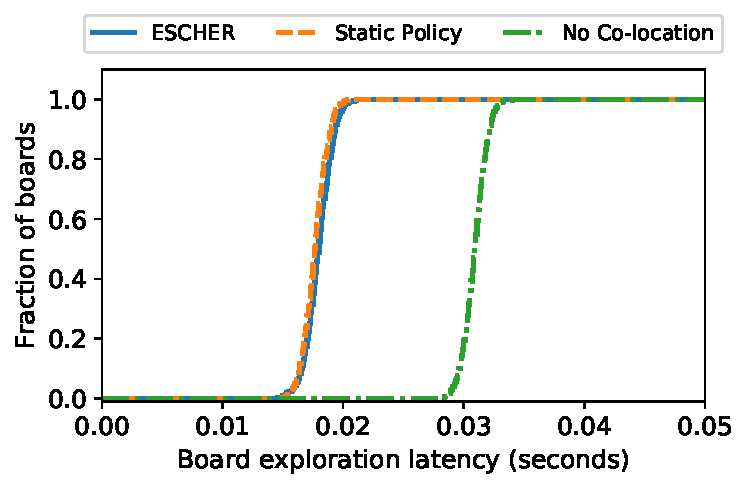
\includegraphics[width=\textwidth]{escher/plots/results_e2e_alphago_latencycdf_16node.pdf}
  \caption{}
  \label{fig:alphazerolatencycdf}
\end{subfigure}
\begin{subfigure}[b]{0.26\textwidth}
\centering
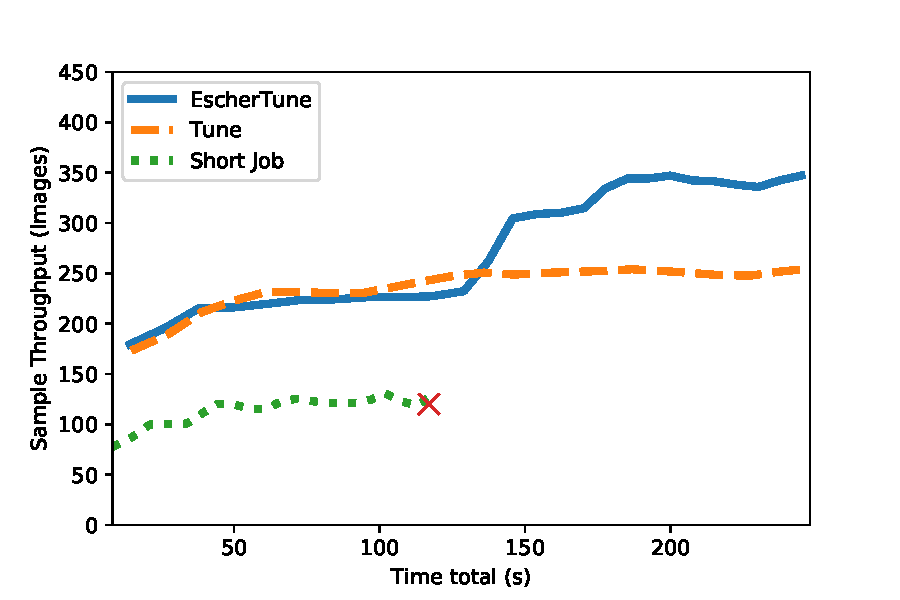
\includegraphics[width=\textwidth,trim=0cm 0cm 1.5cm 0cm, clip]{escher/plots/result_migrationthroughput.pdf}
\caption{}
\label{fig:tune-results}
\end{subfigure}
% \begin{subfigure}[b]{0.3\textwidth}
%   \centering
%   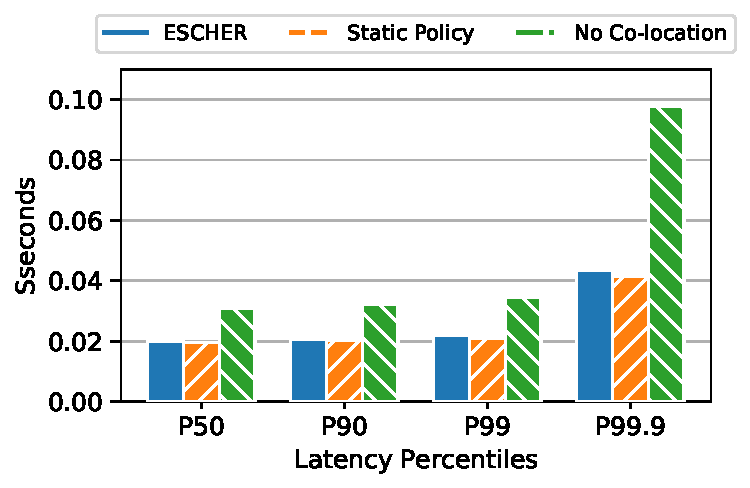
\includegraphics[width=\textwidth]{escher/plots/results_e2e_alphago_pxxcompare_16node.pdf}
%   \caption{}
%   \label{fig:alphazerolatencypxx}
% \end{subfigure}
\caption{\small AlphaZero and distributed training on \name{}. \textbf{(a)} Implementing AlphaZero policy with ESCHER, composing co-location with load-balancing.
% By co-locating the \textit{BoardAggregator}s and the \textit{PredictorAgent}s, the \name{} takes significantly lower time to generate and evaluate board states than an unaware scheduler. \name{} also performs comparably with a static policy that hard codes placement decisions, while offering the flexibility of a general scheduling policy.
\textbf{(b)} A CDF of AlphaZero board exploration latency, and
\textbf{(c)} Throughput comparison of a distributed training workload with a mix of short-running and long-running jobs. EscherTune is an augmentation of the hyperparameter search framework Tune~\cite{liaw2018tune}, using ESCHER to dynamically re-schedule jobs as others complete. %SCHER augments an existing application, Tune, to increase sample throughput. 
The red X indicates the completion of a short job. %, and EscherTune re-schedules the long-running job to claim the idle resources. % to utilize the co-location mechanism and decrease communication overhead compared to Tune.
}
\label{fig:alphazerolatencyfigure}
\vspace{-2mm}
\end{figure*}


\begin{figure}[t]
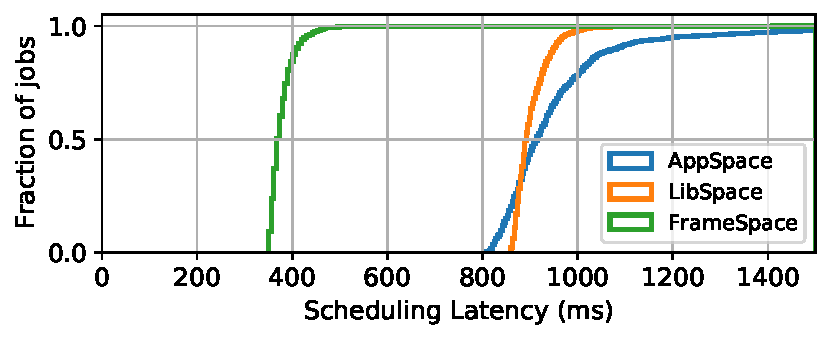
\includegraphics[width=0.92\columnwidth]{escher/plots/result_gangsched_design_compare.pdf}
\caption{\small Request latency for gang scheduling implemented in the application space, with (\textit{LibSpace}) and without (\textit{AppSpace}) coordination, versus the framework space (\textit{FrameSpace}). \textit{FrameSpace} is 1624 lines of code (LoC), \textit{LibSpace} with 261 LoC and \textit{AppSpace} with 78 LoC.}
\label{fig:gangscheddesign-results}
\end{figure}

\subsection{Microbenchmarks}
\subsubsection{Overhead of application-level policies}
\label{sec:eval:gangscheduling}
ESCHER scheduling policies can be implemented either in the application space for evolvability or in the framework for performance.
We evaluate the trade-offs involved in this choice by comparing three distinct designs of gang scheduling, all with ephemeral resources on Ray.

\textit{AppSpace} uses ghost tasks to atomically reserve resources (\Cref{policies:gangsched}).
% An application can call this policy without any coordination with another application in the same cluster.
While this policy is simple to integrate, the lack of coordination between applications can lead to deadlock, which must be resolved through timeouts. %it uses expensive ghost tasks to reserve resources and must resolve any livelocks through expensive timeouts.
\textit{LibSpace} avoids this by using a \emph{shared library}: a shared service in the cluster that serializes gang scheduling requests across applications.
% An application using \textit{LibSpace} sends all gang scheduling requests to this service, which returns the set of ephemeral resources that should be specified when submitting tasks.
\textit{LibSpace} thus avoids live lock entirely but requires deploying a separate shared service.
% \textit{LibSpace} improves upon this by using the same ghost task approach, but in a shared library which runs as a common service in the cluster to provide inter-job coordination. All jobs must communicate with this library to request gang scheduling of their tasks by specifying the resources required for scheduling all tasks. The library returns a ephemeral resource that must then be used by the application to place its tasks. \textit{LibSpace} is able to serialize gang scheduling across jobs, allowing it to avoid live-locks.
Finally, \textit{FrameSpace} modifies the Ray scheduler to expose a gang scheduling API.
Internally, a centralized service within Ray directly reserves and creates ephemeral resources.
Since it has direct access to the resource table, \textit{FrameSpace} avoids using ghost tasks, reducing overheads from worker allocation and task dispatch.

% implements gang scheduling as a part of the core Ray scheduler. This requires modifications in the core ray scheduler to expose an API for applications to request gang scheduling of their tasks. Internally, this implementation directly reserves resources in the scheduler's resource availability map and creates an ephemeral resource which is returned and requested by tasks to schedule their gang of tasks. 

\Cref{fig:gangscheddesign-results} compares the request latency of these designs on a 32-node cluster with 256 CPUs.
% We subsample 100k gang-scheduling requests from the Google ClusterData 2011 trace~\cite{clusterdata:Reiss2011}. % and measure the scheduling latency per request. %and measure the time taken from request submission to job start (scheduling latency).
% We subsample the Google ClusterData 2011 trace \cite{clusterdata:Reiss2011} to model request arrival patterns. 
% To evaluate the performance of these designs, we set up a cluster of 32 nodes with 8 CPUs each. We then submit 100k gang-scheduling requests over 15 minutes and measure the scheduling latency per request. %and measure the time taken from request submission to job start (scheduling latency).
% We subsample the Google ClusterData 2011 trace \cite{clusterdata:Reiss2011} to model request arrival patterns. Figure \ref{fig:gangscheddesign-results} compares the scheduling latency across the three designs.
While the mean latency of \textit{AppSpace} and \textit{LibSpace} is similar, \textit{AppSpace} has higher variance and a longer tail because it uses timeouts to break deadlocks.
\textit{LibSpace} incurs overhead from serializing requests at a separate service, resulting in a higher minimum latency. On average, \textit{FrameSpace} is nearly $2\times$ faster than \textit{AppSpace} and \textit{LibSpace} because it directly reserves resources instead of using ghost tasks. However, we note that for long-running tasks such as model training and batch processing workloads, the absolute scheduling latency is still a tiny fraction (<1s) compared to the runtime of the workloads (multiple hours). Moreover, implementing \textit{FrameSpace} is a significant effort, requiring a deep understanding of the Ray scheduler and modifying 1624 lines of Ray code.
To compare, \textit{LibSpace} and \textit{AppSpace} are implemented in 261 and 78 lines of \emph{application-level} code, respectively.



\subsubsection{Overheads of Ephemeral Resources}
% In this section, we evaluate the costs of introducing ephemeral resources in the framework scheduler.


%\textbf{Dynamic resource creation.}
%Scheduling with ephemeral resources relies on the ability to create and modify resources at run-time.
We evaluate the time to create resources and propagate their availability throughout the cluster.
Since the \lstinline{set_resource} call is asynchronous, we verify that the resources have been created and are available for use by launching no-op tasks that request these newly created resources. %The completion of these tasks marks the successful creation and propagation of ephemeral resources.
% \begin{figure}
%     \centering
%     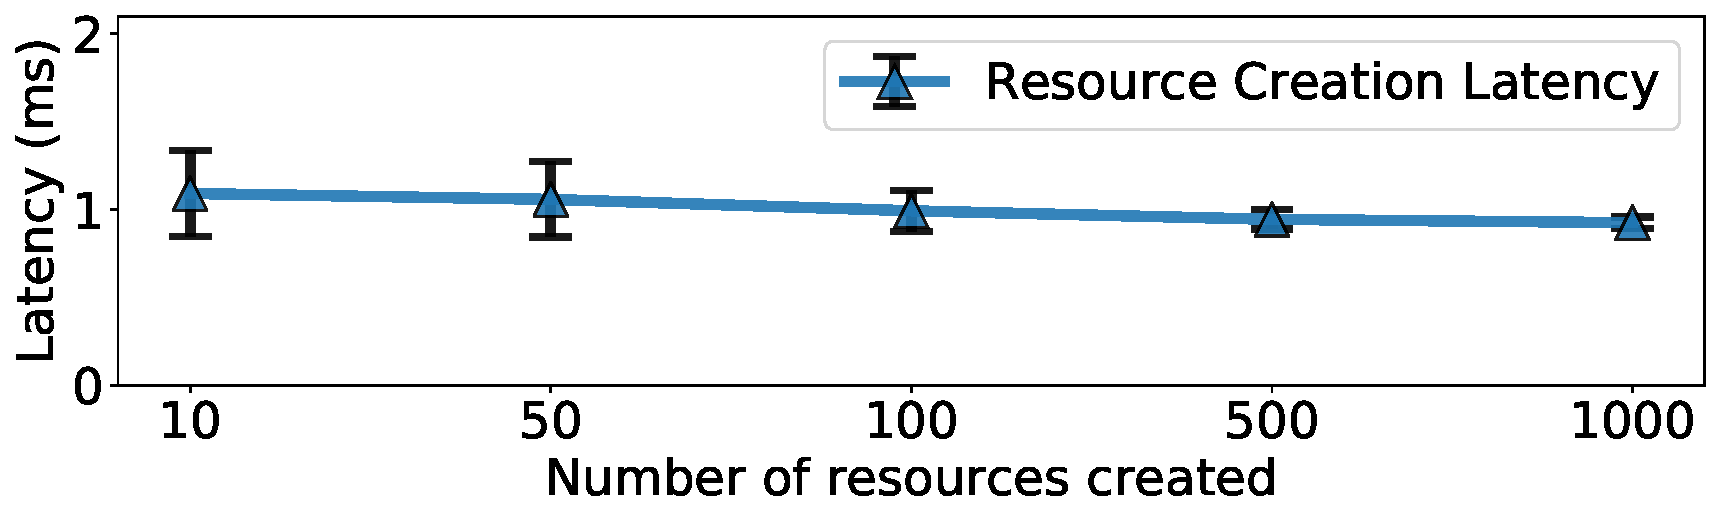
\includegraphics[width=\linewidth]{escher/plots/result_microbench_creationlatency_vs_numres.pdf}
%     \caption{\small Mean per-resource creation latency in Ray. Creating ephemeral resources in \name{} is a low cost operation that scales linearly with the number of resources created.}
%     \label{fig:res-creation-microbench}
% \end{figure}
Figure \ref{fig:res-creation-microbench} compares the mean latency of creating an equal number of resources on each node in a 50-node \ray{} cluster.
We show that even when creating 1000 ephemeral resources, we can maintain 1ms latency per request.
% against the number of resources created using the \lstinline{set_resource} API.
%Number of resources reflects the total resources created in the cluster, while the mean time to resource creation is measured as the time taken from the \lstinline{set_resource} submission to the availability of the resource.
As more resources are created, the cost of resource creation is amortized and the per-resource creation cost decreases to 0.72ms. 
In general, the overhead of creating or deleting an ephemeral resource should be roughly equivalent to that of a key-value store request.
% In absolute terms, the cost of creating ephemeral resources is insignificant, making \name{} a viable design.



\begin{figure*}[t]
\centering
\begin{subfigure}[b]{0.31\linewidth}
  \centering
  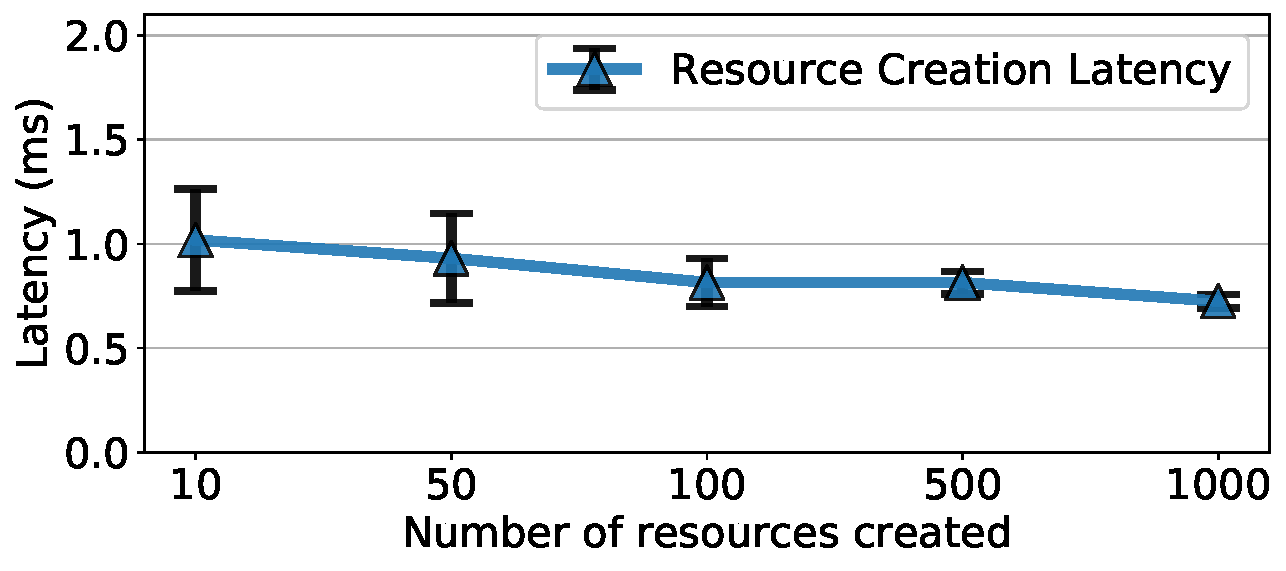
\includegraphics[width=\textwidth]{escher/plots/microbench_horz/result_microbench_creationlatency_vs_numres_horz.pdf}
  \caption{}
  \label{fig:res-creation-microbench}
\end{subfigure}
\begin{subfigure}[b]{0.31\textwidth}
  \centering
  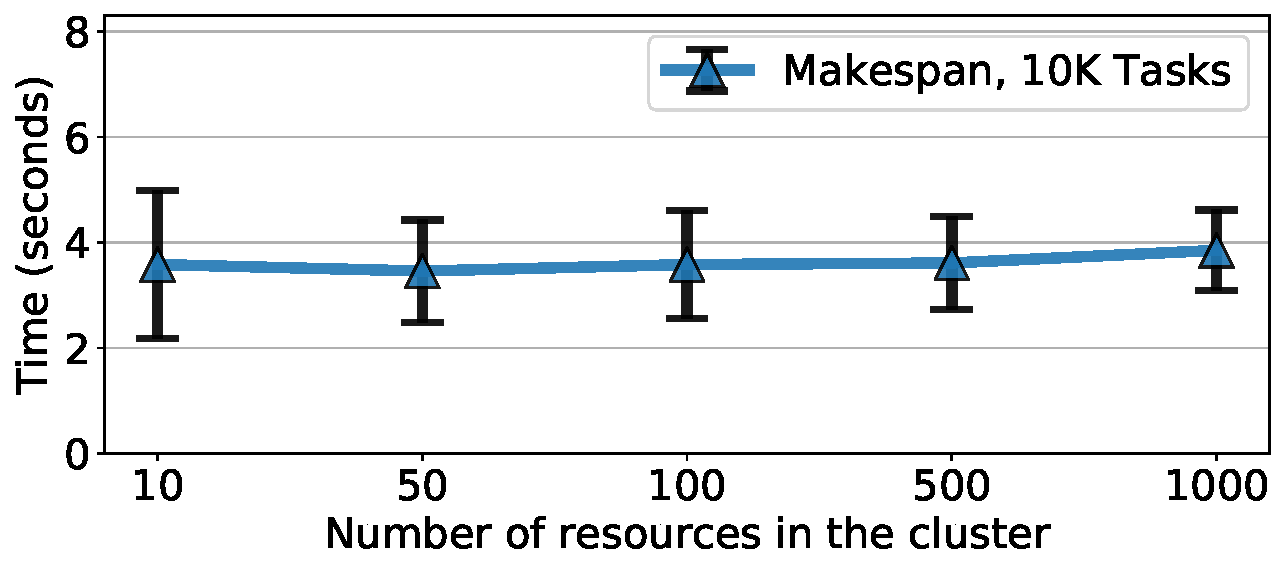
\includegraphics[width=\textwidth]{escher/plots/microbench_horz/result_microbench_schedlatency_vs_clusterresources_horz.pdf}
  \caption{}
  \label{fig:schedlatency-resources-microbench}
\end{subfigure}
\begin{subfigure}[b]{0.31\textwidth}
  \centering
  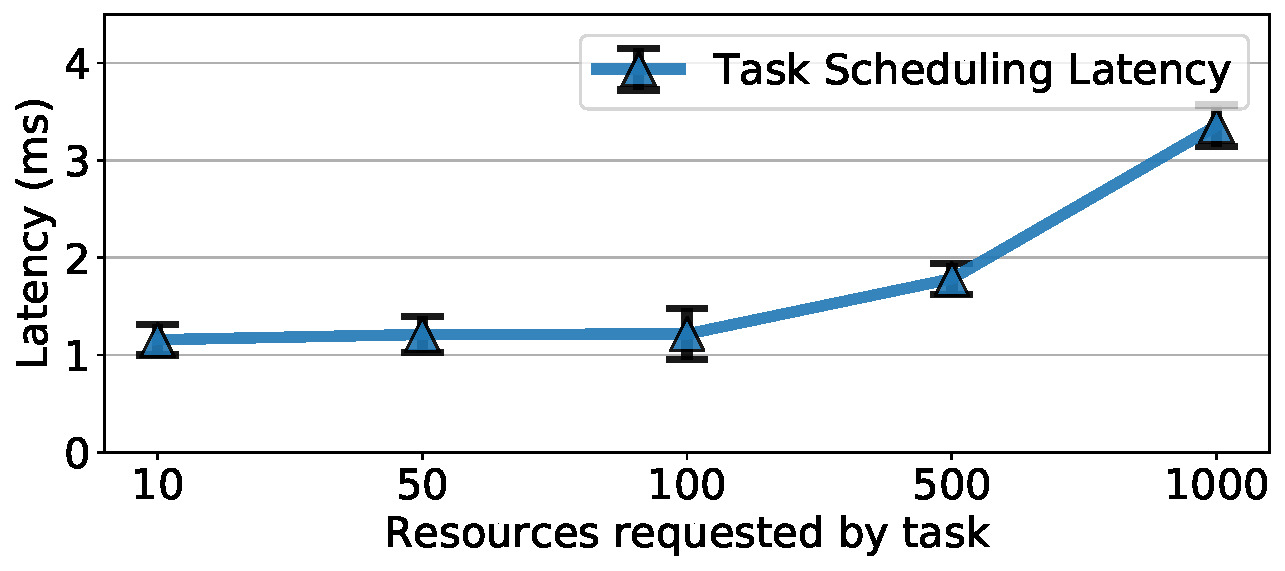
\includegraphics[width=\textwidth]{escher/plots/microbench_horz/result_microbench_schedlatency_vs_resrequested_horz.pdf}
  \caption{}
  \label{fig:schedlatency-taskrequest-microbench}
\end{subfigure}
\vspace{-4mm}
\caption{\small \name{} microbenchmarks. \textbf{(a)} Mean per-resource creation latency in Ray. Creating ephemeral resources in \name{} is a low-cost operation that scales linearly with the number of resources created. \textbf{(b)} Scheduling latency overheads from presence of ephemeral resources. Makespan of a 10000 task workload remains unaffected by the count of ephemeral resources in the cluster. \textbf{(c)} Effect of task resource requirements on scheduling latency in an environment with 10000 resources.}
\label{fig:microbenchfig}
\end{figure*}


\noindent\textbf{Ephemeral resources and scheduling latency.}
%The core task of the framework scheduler is to match task resource requirements with cluster resource availability.
The creation of ephemeral resources may add burden to the scheduler, as it must consider a greater number of attributes during resource matching.
% The usage of ephemeral resources imposes an additional burden on the scheduler and its resource matching complexity, as the number of resource attributes managed by the scheduler and the dimensionality of compared resource attribute vectors grows. 
Therefore, we analyze the effect of resource creation on task scheduling latency. We create an equal number of resources across 50 \ray{} nodes in a cluster using the \lstinline{set_resource} API. We then evaluate two cases based on the resource requirements of the tasks involved.

% \textbf{Tasks without resource requirements.}
First, in Figure~\ref{fig:schedlatency-resources-microbench}, we launch 10,000 tasks, none of which require any ephemeral resources to be scheduled. %, and measure the makespan of this workload against the number of resources present in the cluster.
As the tasks do not have any specific resource requirements, the scheduler execution time and workload makespan are not affected by the number of ephemeral resources present. %, and the makespan of the workload remains unaffected even by the presence of other ephemeral resources in the cluster.

% we highlight the effects of presence of ephemeral resources on scheduling latency for tasks that do not make use of ephemeral resources. In this microbenchmark, we launch a workload of 10k tasks, none of which require any ephemeral resources to be scheduled and compare the makespan of this workload against the number of resources present in the cluster. As the tasks do not have any specific resource requirements, the scheduler execution time remains constant, and the makespan of the workload remains unaffected even by the presence of other ephemeral resources in the cluster.
        % \begin{figure}
        %     \centering
        %     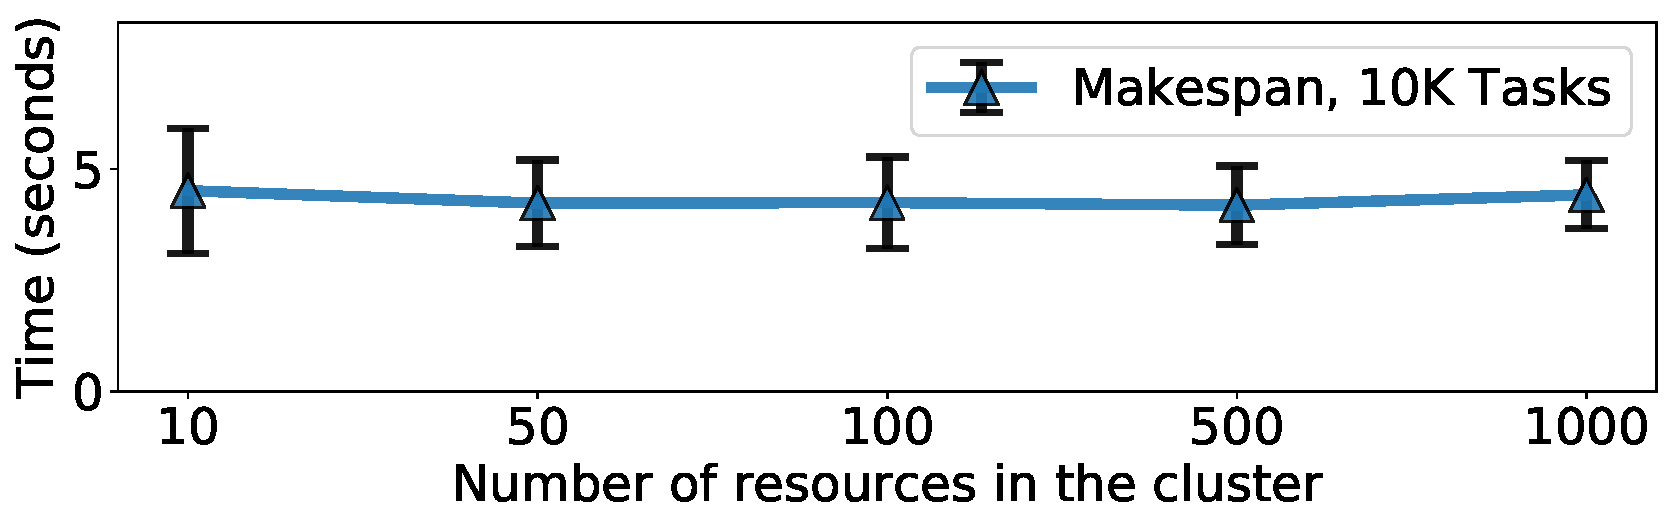
\includegraphics[width=\linewidth]{escher/plots/result_microbench_schedlatency_vs_clusterresources.pdf}
        %     \caption{\small Scheduling latency overheads from presence of ephemeral resources.  The makespan of a  10000 task workload remains unaffected by the count of ephemeral resources present in the cluster. }
        %     \label{fig:schedlatency-resources-microbench}
        %     \vspace{-4mm}
        % \end{figure}
        
% \textbf{Tasks with resource requirements.}
Second, when tasks do request ephemeral resources, the core scheduler must match the task's requirements to a set of candidate nodes.
To evaluate the overheads introduced by this matching, we setup a 50 node \ray{} cluster and create 1000 unique ephemeral resources evenly spread across nodes.
Figure 8c highlights the scalability of the scheduler as the number of ephemeral resources requested by a task grows. The the task scheduling latency grows only from 1.1ms to 1.2ms when requesting 1 vs. 100 ephemeral resources, respectively. We note that all policies described in this work require only a few ephemeral resources to express.
% We then perform multiple trials that launch a no-op task that requests a range from 10 to 1000 distinct resources.
%Figure \ref{fig:schedlatency-taskrequest-microbench} shows the scheduling latency of a no-op task against the number of resource requested by the task. The scheduling latency remains constant up to requests as large as 100 resources. Note that even the most complex scheduling policies do not require more than a few ephemeral resources.
    
        % \begin{figure}
        %     \centering
        %     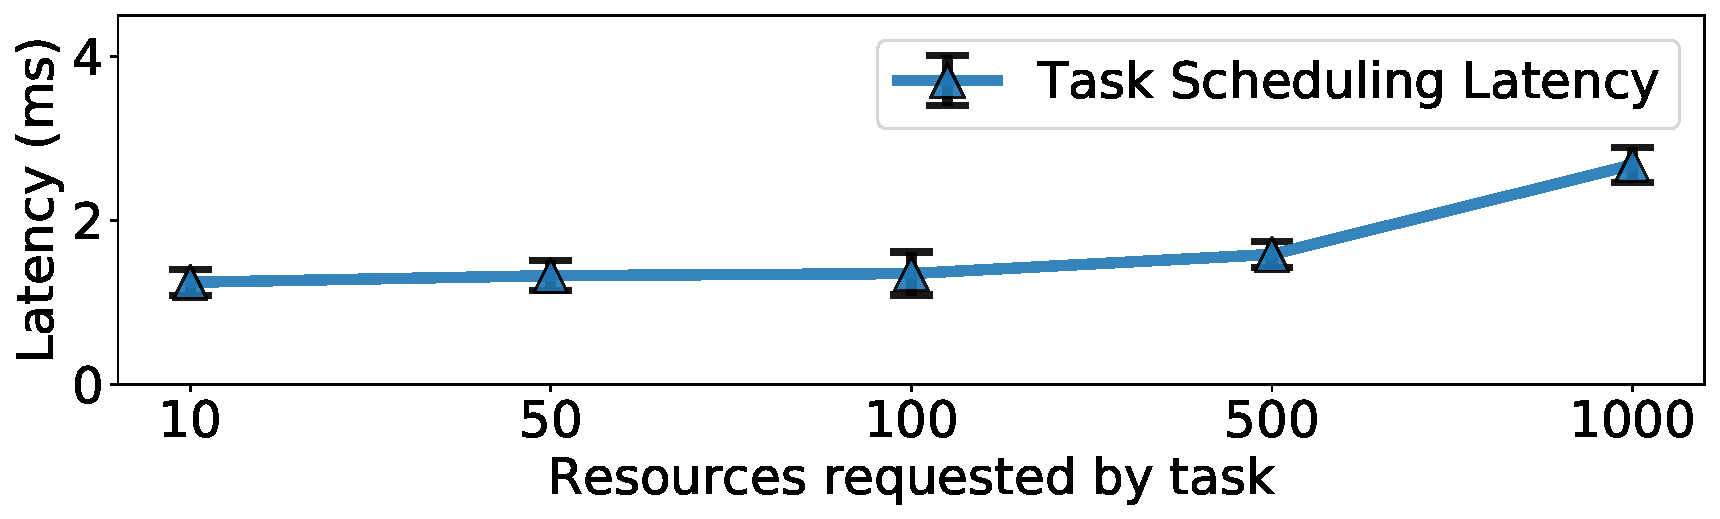
\includegraphics[width=\linewidth]{escher/plots/result_microbench_schedlatency_vs_resrequested.pdf}
        %     \caption{\small Effect of task resource requirements on scheduling latency in an environment with 10000 resources spread over 10 nodes. As a task resource requests more resources, the scheduling latency increases, but even the most complex scheduling policies do not require more than tens of resources. }
        %     \label{fig:schedlatency-taskrequest-microbench}
        % \end{figure}


% \textbf{Value of Locality-Aware scheduling.} In this microbenchmark, we study the motivation for co-location of tasks with the data they operate on. Specifically, we aim to evaluate the network cost of placing tasks and data on separate physical machines. We create arrays of varying sizes across 2 nodes in a \ray{} cluster and run two sets of tasks which fetch the data and perform a no-op. The first set of tasks uses ephemeral resources to co-locate with the data each task works on, while the other set of tasks is randomly placed.

% Figure \ref{fig:locality-latency} compares the task latency when tasks are co-located against random placement. \textcolor{red}{These numbers will be more dramatic soon - this run is local on one machine. Also, Is this a useful microbenchmark?}.

%     \begin{figure}
%         \centering
%         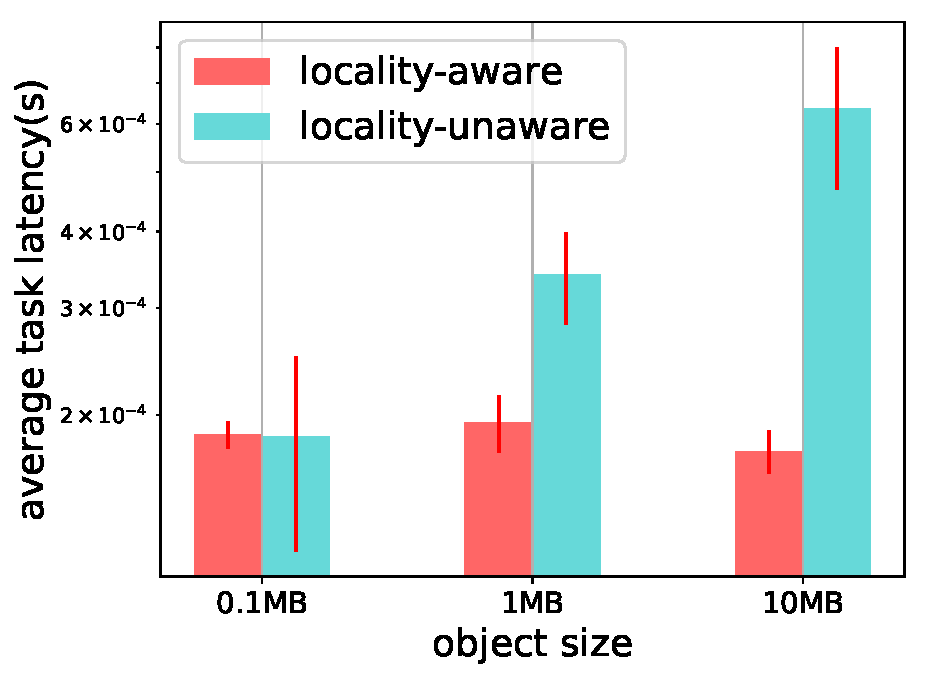
\includegraphics[width=\linewidth]{locality-latency.pdf}
%         \caption{Task-latency - Data-locality vs object size.}
%         \label{fig:locality-latency}
%     \end{figure}

% \subsection{Discussion}
% \textbf{Performance-evolvability tradeoff.} As we implemented our evaluation workloads, we found that \name{} significantly reduced the effort to express the workloads' scheduling constraints. In the AlphaZero workload, it required only 5 lines of code to be changed to express a composition of load-balancing and co-location. Implementing the same policy in Ray would have required re-writing the scheduler to enforce this policy on all tasks, since there is no policy selection mechanism in Ray. Same was true for implementing Gang Scheduling.

% However, as we see in the Gang Scheduling microbenchmark, the ghost task mechanism introduces latency due to the back-off performed by each ghost task on failure. While this latency is insignificant for long-running tasks, such as in distributed training, we acknowledge that this is a natural tradeoff ESCHER makes. It sacrifices performance for certain policies in favor of significantly reducing the implementation burden at the application-level. This gain in evolvability can be valuable for many applications, for whom functionality in the short-term (while the policy is integrated into the scheduler) may be more important than performance. 

% \textbf{Debugging ESCHER policies.} Since ephemeral resources are declarative in nature, debugging them requires replay of resource creation/deletion logs, which can be challenging.
